\documentclass[../../main.tex]{subfiles}

\begin{document}
\chapter{Planificación y presupuesto}
\label{C:planificacion}

La planificación del proyecto constituye una etapa fundamental para garantizar un desarrollo ordenado y coherente del sistema. En este capítulo se describe la organización temporal de las distintas tareas, así como la estructuración del trabajo en fases claramente diferenciadas. Esta planificación ha permitido establecer una guía de referencia durante el desarrollo, facilitando la gestión del tiempo, la priorización de objetivos y el seguimiento del progreso del proyecto.

\section{Planificación}
En la Figura \ref{fig:diagrama_gantt} se presenta la planificación temporal del proyecto mediante un diagrama de Gantt, en el que se reflejan las distintas fases y la distribución del trabajo a lo largo del desarrollo.

\begin{figure}[!htb]
    \centering
    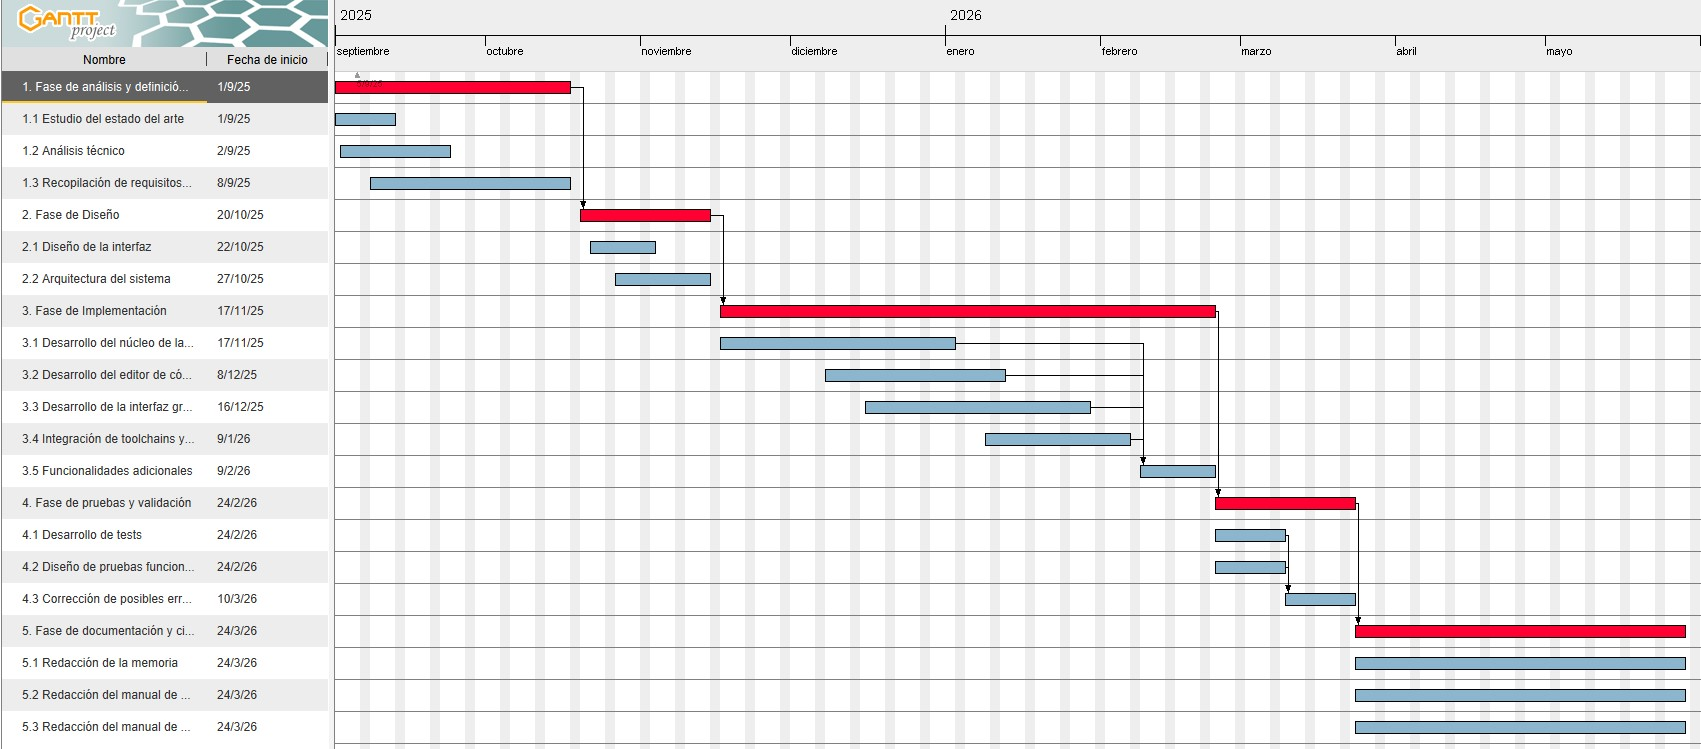
\includegraphics[width=18cm]{../imagenes/diagramas/gantt.jpg} 
    \caption{Diagrama de Gantt del proyecto.}
    \label{fig:diagrama_gantt} 
\end{figure}

\clearpage

Para estructurar el proceso, el proyecto se ha organizado en varias etapas diferenciadas, cada una con objetivos y actividades específicas:

\begin{itemize}
    \item \textbf{Fase de análisis y definición de requisitos:}: corresponde al inicio del proyecto e incluye el estudio del estado del arte, la recopilación de información relevante y la identificación de los requisitos funcionales y técnicos que debía cumplir el sistema.
    \item \textbf{Fase de diseño:} en esta etapa se definió la arquitectura de la aplicación, así como la estructura de sus principales componentes. También se tomaron decisiones relacionadas con las tecnologías a emplear y la organización interna del sistema.
    \item \textbf{Fase de implementación:} comprende el desarrollo del sistema, incluyendo tanto la construcción de la interfaz de usuario como la integración de las distintas funcionalidades, tales como la edición de código, la compilación y la ejecución en emuladores.
    \item \textbf{Fase de pruebas y validación:} se realizaron pruebas para verificar el correcto funcionamiento de la aplicación, detectando y corrigiendo errores, así como comprobando que los requisitos definidos inicialmente se cumplían de forma adecuada.
    \item \textbf{Fase de documentación y cierre:} etapa final del proyecto en la que se ha llevado a cabo la elaboración de la memoria, la preparación del manual de usuario y la revisión global del sistema antes de su entrega.
\end{itemize}

A continuación, se describen en detalle cada una de estas fases.
 
\subsection{Fase de análisis y definición de requisitos}

Durante la fase de análisis y definición de requisitos se llevó a cabo un estudio exhaustivo del estado del arte en el ámbito de los entornos de desarrollo integrados (IDEs) para sistemas embebidos. Se observaron las fortalezas y debilidades de las herramientas ya existentes y se identificaron los puntos comunes y qué puntos se podrían mejorar.

Se recopilaron y analizaron diversas fuentes de información, incluyendo documentación técnica, y proyectos similares, con el objetivo de identificar las mejores prácticas y las tecnologías más adecuadas para el desarrollo del sistema. 

También se definieron los requisitos funcionales y técnicos que debía cumplir la aplicación con toda la información recopilada. 

\clearpage
  
Como se puede observar en la Figura \ref{fig:diagrama_gantt_fase_analisis}, esta fase se extendió durante las primeras semanas del proyecto, permitiendo establecer una base sólida para las etapas posteriores.
\begin{figure}[!htb]
    \centering
    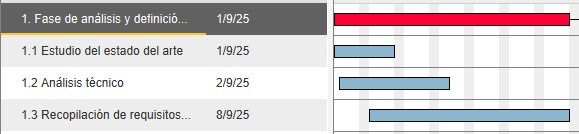
\includegraphics[width=12cm]{../imagenes/diagramas/gantt_analisis.jpg} 
    \caption{Diagrama de Gantt de la fase de análisis y definición de requisitos.}
    \label{fig:diagrama_gantt_fase_analisis} 
\end{figure}



Las subtareas de esta fase incluyeron:

\begin{itemize}
    \item \textbf{1.1 Estudio del estado del arte:} se llevó a cabo una investigación detallada sobre las herramientas y tecnologías existentes en el ámbito de los IDEs para sistemas retro, identificando sus características, ventajas y limitaciones.
    \item \textbf{1.2 Análisis técnico:} se evaluaron las diferentes opciones tecnológicas y se determinaron las más adecuadas para el desarrollo del sistema.
    \item \textbf{1.3 Recopilación de requisitos funcionales:} se definieron los requisitos que debía cumplir la aplicación, basándose en la información recopilada y en las necesidades del usuario.
\end{itemize}

Esta fase fue crucial para garantizar que el desarrollo se orientara hacia la creación de un producto que alcanzara los objetivos establecidos.


\subsection{Fase de diseño} 

Durante la fase de diseño se definió la arquitectura general del sistema, estableciendo los principales componentes y su interacción. Se diseñó la estructura de la aplicación, incluyendo la organización de las interfaces de usuario, los módulos de procesamiento y las herramientas de integración. Además, se tomaron decisiones clave sobre las tecnologías a emplear, asegurando que fueran adecuadas para cumplir con los requisitos funcionales y técnicos establecidos en la fase anterior. 

Este diseño detallado sirvió como base para la posterior implementación del sistema, proporcionando una guía clara para el desarrollo y facilitando la identificación de posibles desafíos o áreas de mejora desde el inicio del proceso.

\clearpage

Para el desarrollo de esta fase se asignaron varias semanas, como se muestra en la Figura \ref{fig:diagrama_gantt_fase_diseno}.

\begin{figure}[!htb]
    \centering
    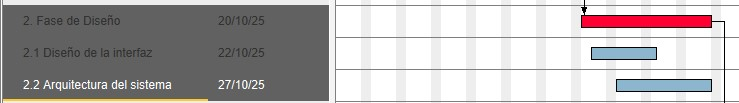
\includegraphics[width=12cm]{../imagenes/diagramas/gantt_diseno.jpg} 
    \caption{Diagrama de Gantt de la fase de diseño.}
    \label{fig:diagrama_gantt_fase_diseno} 
\end{figure}

Las subtareas de esta fase incluyeron:

\begin{itemize}
    \item \textbf{2.1 Diseño de la interfaz:} se definió la apariencia y la disposición de los elementos de la interfaz de usuario, asegurando una experiencia intuitiva y coherente.
    \item \textbf{2.2 Arquitectura del sistema:} se estableció la estructura general del sistema, incluyendo los módulos principales y sus interacciones, garantizando una base sólida para la implementación.
\end{itemize}


\subsection{Fase de implementación}

Durante la fase de implementación se llevó a cabo el desarrollo del sistema, siguiendo las especificaciones y el diseño definidos en las etapas anteriores. Se implementaron las distintas funcionalidades de la aplicación, incluyendo la edición de código, la compilación y la ejecución en emuladores. Además, se integraron las toolchains necesarias para el correcto funcionamiento del sistema, asegurando que todas las partes del proyecto trabajaran de manera coherente y eficiente. 

Durante esta etapa, se realizaron ajustes y mejoras continuas para garantizar que el producto final cumpliera con los requisitos establecidos y ofreciera una experiencia de usuario satisfactoria.

Para el desarrollo de esta fase se asignaron varias semanas, como se muestra en la Figura \ref{fig:diagrama_gantt_fase_implementacion}.

\begin{figure}[!htb]
    \centering
    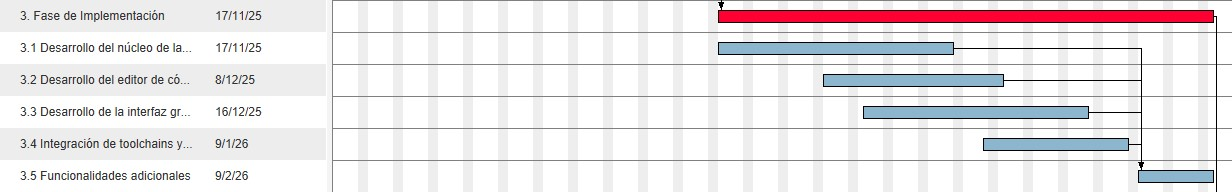
\includegraphics[width=12cm]{../imagenes/diagramas/gantt_implementacion.jpg} 
    \caption{Diagrama de Gantt de la fase de implementación.}
    \label{fig:diagrama_gantt_fase_implementacion} 
\end{figure}

Las subtareas de esta fase incluyeron:

\begin{itemize}
    \item \textbf{3.1 Desarrollo del núcleo de la aplicación:} se implementaron las funcionalidades principales del sistema, asegurando su correcto funcionamiento y eficiencia.
    \item \textbf{3.2 Desarrollo del editor de código:} se creó un entorno de edición de código integrado, con soporte para resaltado de sintaxis.
    \item \textbf{3.3 Desarrollo de la interfaz gráfica:} se diseñó y desarrolló la interfaz de usuario, garantizando una experiencia intuitiva y coherente.
    \item \textbf{3.4 Integración de toolchains y emuladores:} se incorporaron las herramientas necesarias para la compilación y ejecución del código en diferentes entornos.
    \item \textbf{3.5 Funcionalidades adicionales:} se añadieron características complementarias como el sistema de plugins y la personalización de la interfaz.
\end{itemize}


\subsection{Fase de pruebas y validación}

En esta fase se llevaron a cabo pruebas exhaustivas para garantizar la calidad y el correcto funcionamiento del sistema. 

Se realizaron pruebas unitarias para verificar el comportamiento de cada componente de forma individual. Además, se llevaron a cabo pruebas funcionales para validar que el sistema cumplía con los requisitos definidos inicialmente. 

Durante esta etapa, se identificaron y corrigieron diversos errores y se realizaron ajustes para mejorar la estabilidad y el rendimiento del sistema.

Para el desarrollo de esta fase se asignó un tiempo razonable para poder completar todas las pruebas necesarias, como se muestra en la Figura \ref{fig:diagrama_gantt_fase_pruebas}.

\begin{figure}[!htb]
    \centering
    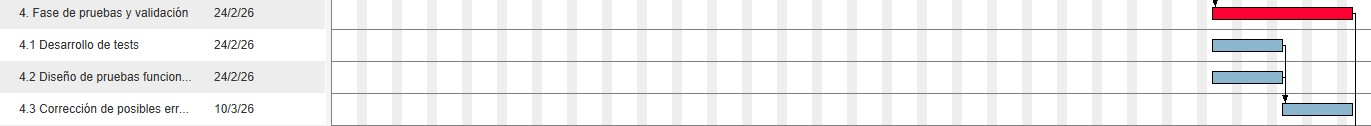
\includegraphics[width=12cm]{../imagenes/diagramas/gantt_pruebas.jpg} 
    \caption{Diagrama de Gantt de la fase de pruebas y validación.}
    \label{fig:diagrama_gantt_fase_pruebas} 
\end{figure}

Las subtareas de esta fase incluyeron:

\begin{itemize}
    \item \textbf{4.1 Pruebas unitarias:} se verificó el correcto funcionamiento de cada componente de forma individual, asegurando que cumplían con sus especificaciones.
    \item \textbf{4.2 Pruebas funcionales:} se validó que el sistema cumplía con los requisitos definidos inicialmente, comprobando su comportamiento en diferentes escenarios de uso.
    \item \textbf{4.3 Corrección de errores:} se identificaron y corrigieron diversos errores detectados durante las pruebas, mejorando la estabilidad y el rendimiento del sistema.
\end{itemize}

Es importante observar que el punto 4.3 es dependiente de los resultados obtenidos en los puntos 4.1 y 4.2.

Cabe destacar la criticidad para el proyecto de esta fase, ya que el diseño de unos test adecuados y la identificación temprana de errores son fundamentales para garantizar un proyecto robusto y de calidad.

\clearpage

\subsection{Fase de documentación y cierre}

En la fase de documentación y cierre se llevó a cabo la elaboración de la memoria del proyecto, que incluye una descripción detallada del desarrollo, los resultados obtenidos y las conclusiones finales. Además, se preparó un manual de usuario para facilitar la comprensión y el uso de la aplicación por parte de los usuarios finales y un manual de desarrollo de plugins para que un usuario pueda crear y gestionar sus propios complementos de manera eficiente.

Durante esta etapa, se realizó una revisión global del sistema para identificar posibles mejoras y se llevaron a cabo ajustes finales antes de la entrega del proyecto. 

Se precisó para ello mas de dos meses, como se muestra en la Figura \ref{fig:diagrama_gantt_fase_documentacion}, debido a que esta tarea implica la recopilación de toda la información generada durante el desarrollo del proyecto.

\begin{figure}[!htb]
    \centering
    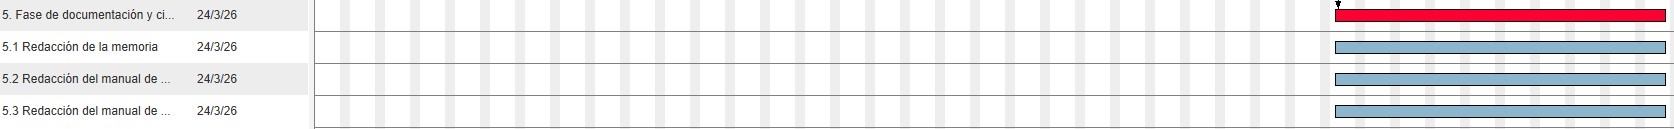
\includegraphics[width=12cm]{../imagenes/diagramas/gantt_documentacion.jpg} 
    \caption{Diagrama de Gantt de la fase de documentación y cierre.}
    \label{fig:diagrama_gantt_fase_documentacion}   
\end{figure}

\section{Presupuesto}

A continuación, se presenta una estimación económica del proyecto, sin incluir el Impuesto sobre el Valor Añadido (IVA). Dicha estimación se ha realizado tomando como referencia la planificación definida en el anteproyecto, en la que el desarrollo se estructura en fases secuenciales siguiendo un modelo en cascada.

\begin{center}
\begin{tabular}{|l|c|c|c|}
\hline
\textbf{Fase} & \textbf{Horas} & \textbf{€/hora} & \textbf{Coste (€)} \\
\hline
Recopilación de información y formación inicial & 70 & 18 & 1260 \\
\hline
Análisis del sistema & 50 & 20 & 1000 \\
\hline
Diseño del sistema & 40 & 22 & 880 \\
\hline
Implementación del sistema & 150 & 20 & 3000 \\
\hline
Integración de toolchains y emuladores & 60 & 22 & 1320 \\
\hline
Pruebas y validación & 30 & 20 & 600 \\
\hline 
Elaboración de la memoria & 25 & 18 & 450 \\
\hline
\textbf{Total} & \textbf{425} & & \textbf{8.510} \\
\hline
\end{tabular}
\end{center}

\textbf{Tabla X.} Estimación económica del proyecto.

\end{document}